\begin{figure}[h] 
\centering 
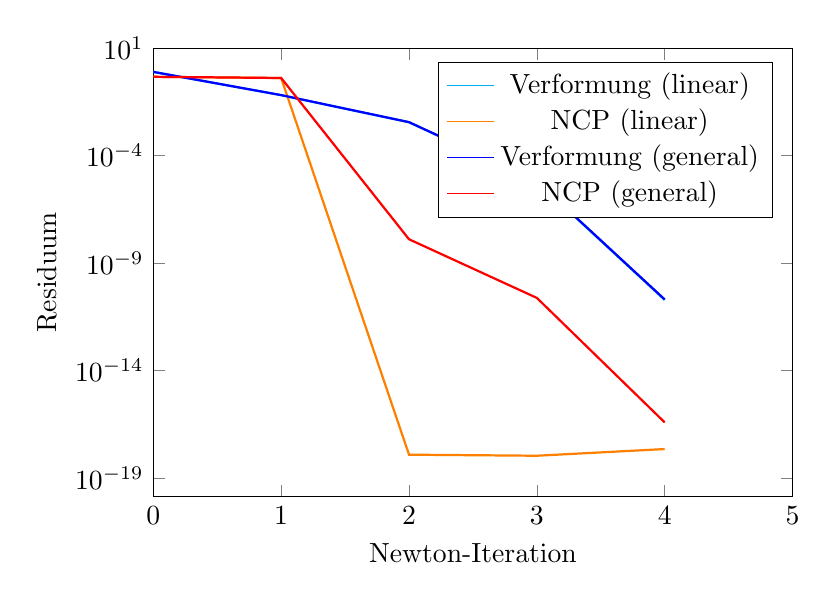
\begin{tikzpicture}[every plot/.append style={thick}] 
\begin{axis}[ 
label style={font=\normalsize}, 
xlabel={Newton-Iteration}, 
ylabel={Residuum}, 
xmin=0, xmax=5, 
ymode=log, 
ymin=0, ymax=10, 
width=0.8\textwidth, 
height=0.6\textwidth, 
legend pos=north east, 
legend style={cells={align=left}}, 
grid style=dashed, 
] 
\addplot[ 
color=cyan, 
] 
coordinates { 
(0, 7.86e-01)(1, 6.51e-02)(2, 3.58e-03)(3, 6.27e-06)(4, 1.94e-11)}; 
\addlegendentry{Verformung (linear)} 
\addplot[ 
color=orange, 
] 
coordinates { 
(0, 4.65e-01)(1, 4.08e-01)(2, 1.23e-18)(3, 1.10e-18)(4, 2.25e-18)}; 
\addlegendentry{NCP (linear)} 
\addplot[ 
color=blue, 
] 
coordinates { 
(0, 7.86e-01)(1, 6.56e-02)(2, 3.62e-03)(3, 6.45e-06)(4, 2.05e-11)}; 
\addlegendentry{Verformung (general)} 
\addplot[ 
color=red, 
] 
coordinates { 
(0, 4.65e-01)(1, 4.10e-01)(2, 1.29e-08)(3, 2.41e-11)(4, 3.90e-17)}; 
\addlegendentry{NCP (general)} 
\end{axis} 
\end{tikzpicture} 
\caption{Residuen des Stoffgesetzes 'St.Venant' mit Hinderniss 'Parabel' und 578 Freiheitsgraden für die Verschiebung.} 
\label{fiq:St.Venant_Parabel_level3} 
\end{figure} 
